% Created by tikzDevice version 0.11 on 2018-07-30 13:33:02
% !TEX encoding = UTF-8 Unicode
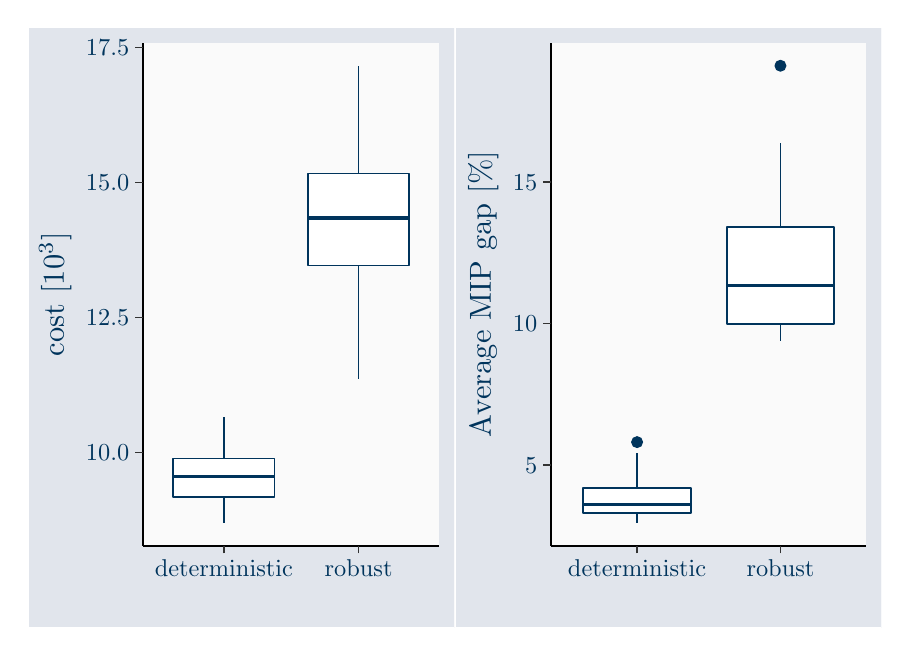
\begin{tikzpicture}[x=1pt,y=1pt]
\definecolor{fillColor}{RGB}{255,255,255}
\path[use as bounding box,fill=fillColor,fill opacity=0.00] (0,0) rectangle (308.59,216.81);
\begin{scope}
\path[clip] (  0.00,  0.00) rectangle (154.30,216.81);
\definecolor{drawColor}{RGB}{255,255,255}
\definecolor{fillColor}{RGB}{225,229,236}

\path[draw=drawColor,line width= 0.6pt,line join=round,line cap=round,fill=fillColor] (  0.00,  0.00) rectangle (154.30,216.81);
\end{scope}
\begin{scope}
\path[clip] ( 41.67, 29.59) rectangle (148.80,211.31);
\definecolor{fillColor}{gray}{0.98}

\path[fill=fillColor] ( 41.67, 29.59) rectangle (148.80,211.31);
\definecolor{drawColor}{RGB}{0,52,92}

\path[draw=drawColor,line width= 0.6pt,line join=round] ( 70.89, 61.17) -- ( 70.89, 76.26);

\path[draw=drawColor,line width= 0.6pt,line join=round] ( 70.89, 47.21) -- ( 70.89, 37.85);
\definecolor{fillColor}{RGB}{255,255,255}

\path[draw=drawColor,line width= 0.6pt,line join=round,line cap=round,fill=fillColor] ( 52.63, 61.17) --
	( 52.63, 47.21) --
	( 89.15, 47.21) --
	( 89.15, 61.17) --
	( 52.63, 61.17) --
	cycle;

\path[draw=drawColor,line width= 1.1pt,line join=round] ( 52.63, 54.77) -- ( 89.15, 54.77);

\path[draw=drawColor,line width= 0.6pt,line join=round] (119.58,164.06) -- (119.58,203.05);

\path[draw=drawColor,line width= 0.6pt,line join=round] (119.58,130.88) -- (119.58, 89.89);

\path[draw=drawColor,line width= 0.6pt,line join=round,line cap=round,fill=fillColor] (101.32,164.06) --
	(101.32,130.88) --
	(137.84,130.88) --
	(137.84,164.06) --
	(101.32,164.06) --
	cycle;

\path[draw=drawColor,line width= 1.1pt,line join=round] (101.32,148.04) -- (137.84,148.04);
\end{scope}
\begin{scope}
\path[clip] (  0.00,  0.00) rectangle (308.59,216.81);
\definecolor{drawColor}{RGB}{0,0,0}

\path[draw=drawColor,line width= 0.6pt,line join=round] ( 41.67, 29.59) --
	( 41.67,211.31);
\end{scope}
\begin{scope}
\path[clip] (  0.00,  0.00) rectangle (308.59,216.81);
\definecolor{drawColor}{RGB}{0,52,92}

\node[text=drawColor,anchor=base east,inner sep=0pt, outer sep=0pt, scale=  0.88] at ( 36.72, 60.32) {10.0};

\node[text=drawColor,anchor=base east,inner sep=0pt, outer sep=0pt, scale=  0.88] at ( 36.72,109.07) {12.5};

\node[text=drawColor,anchor=base east,inner sep=0pt, outer sep=0pt, scale=  0.88] at ( 36.72,157.82) {15.0};

\node[text=drawColor,anchor=base east,inner sep=0pt, outer sep=0pt, scale=  0.88] at ( 36.72,206.58) {17.5};
\end{scope}
\begin{scope}
\path[clip] (  0.00,  0.00) rectangle (308.59,216.81);
\definecolor{drawColor}{gray}{0.20}

\path[draw=drawColor,line width= 0.6pt,line join=round] ( 38.92, 63.35) --
	( 41.67, 63.35);

\path[draw=drawColor,line width= 0.6pt,line join=round] ( 38.92,112.10) --
	( 41.67,112.10);

\path[draw=drawColor,line width= 0.6pt,line join=round] ( 38.92,160.85) --
	( 41.67,160.85);

\path[draw=drawColor,line width= 0.6pt,line join=round] ( 38.92,209.61) --
	( 41.67,209.61);
\end{scope}
\begin{scope}
\path[clip] (  0.00,  0.00) rectangle (308.59,216.81);
\definecolor{drawColor}{RGB}{0,0,0}

\path[draw=drawColor,line width= 0.6pt,line join=round] ( 41.67, 29.59) --
	(148.80, 29.59);
\end{scope}
\begin{scope}
\path[clip] (  0.00,  0.00) rectangle (308.59,216.81);
\definecolor{drawColor}{gray}{0.20}

\path[draw=drawColor,line width= 0.6pt,line join=round] ( 70.89, 26.84) --
	( 70.89, 29.59);

\path[draw=drawColor,line width= 0.6pt,line join=round] (119.58, 26.84) --
	(119.58, 29.59);
\end{scope}
\begin{scope}
\path[clip] (  0.00,  0.00) rectangle (308.59,216.81);
\definecolor{drawColor}{RGB}{0,52,92}

\node[text=drawColor,anchor=base,inner sep=0pt, outer sep=0pt, scale=  0.88] at ( 70.89, 18.58) {deterministic};

\node[text=drawColor,anchor=base,inner sep=0pt, outer sep=0pt, scale=  0.88] at (119.58, 18.58) {robust};
\end{scope}
\begin{scope}
\path[clip] (  0.00,  0.00) rectangle (308.59,216.81);
\definecolor{drawColor}{RGB}{0,52,92}

\node[text=drawColor,rotate= 90.00,anchor=base,inner sep=0pt, outer sep=0pt, scale=  1.10] at ( 13.08,120.45) {cost [$10^3$]};
\end{scope}
\begin{scope}
\path[clip] (154.30,  0.00) rectangle (308.59,216.81);
\definecolor{drawColor}{RGB}{255,255,255}
\definecolor{fillColor}{RGB}{225,229,236}

\path[draw=drawColor,line width= 0.6pt,line join=round,line cap=round,fill=fillColor] (154.30,  0.00) rectangle (308.59,216.81);
\end{scope}
\begin{scope}
\path[clip] (189.12, 29.59) rectangle (303.09,211.31);
\definecolor{fillColor}{gray}{0.98}

\path[fill=fillColor] (189.12, 29.59) rectangle (303.09,211.31);
\definecolor{drawColor}{RGB}{0,52,92}
\definecolor{fillColor}{RGB}{0,52,92}

\path[draw=drawColor,line width= 0.4pt,line join=round,line cap=round,fill=fillColor] (220.21, 67.05) circle (  1.96);

\path[draw=drawColor,line width= 0.6pt,line join=round] (220.21, 50.45) -- (220.21, 62.94);

\path[draw=drawColor,line width= 0.6pt,line join=round] (220.21, 41.42) -- (220.21, 37.85);
\definecolor{fillColor}{RGB}{255,255,255}

\path[draw=drawColor,line width= 0.6pt,line join=round,line cap=round,fill=fillColor] (200.78, 50.45) --
	(200.78, 41.42) --
	(239.63, 41.42) --
	(239.63, 50.45) --
	(200.78, 50.45) --
	cycle;

\path[draw=drawColor,line width= 1.1pt,line join=round] (200.78, 44.35) -- (239.63, 44.35);
\definecolor{fillColor}{RGB}{0,52,92}

\path[draw=drawColor,line width= 0.4pt,line join=round,line cap=round,fill=fillColor] (272.01,203.05) circle (  1.96);

\path[draw=drawColor,line width= 0.6pt,line join=round] (272.01,144.70) -- (272.01,175.16);

\path[draw=drawColor,line width= 0.6pt,line join=round] (272.01,109.71) -- (272.01,103.59);
\definecolor{fillColor}{RGB}{255,255,255}

\path[draw=drawColor,line width= 0.6pt,line join=round,line cap=round,fill=fillColor] (252.58,144.70) --
	(252.58,109.71) --
	(291.44,109.71) --
	(291.44,144.70) --
	(252.58,144.70) --
	cycle;

\path[draw=drawColor,line width= 1.1pt,line join=round] (252.58,123.55) -- (291.44,123.55);
\end{scope}
\begin{scope}
\path[clip] (  0.00,  0.00) rectangle (308.59,216.81);
\definecolor{drawColor}{RGB}{0,0,0}

\path[draw=drawColor,line width= 0.6pt,line join=round] (189.12, 29.59) --
	(189.12,211.31);
\end{scope}
\begin{scope}
\path[clip] (  0.00,  0.00) rectangle (308.59,216.81);
\definecolor{drawColor}{RGB}{0,52,92}

\node[text=drawColor,anchor=base east,inner sep=0pt, outer sep=0pt, scale=  0.88] at (184.17, 55.71) {5};

\node[text=drawColor,anchor=base east,inner sep=0pt, outer sep=0pt, scale=  0.88] at (184.17,106.89) {10};

\node[text=drawColor,anchor=base east,inner sep=0pt, outer sep=0pt, scale=  0.88] at (184.17,158.08) {15};
\end{scope}
\begin{scope}
\path[clip] (  0.00,  0.00) rectangle (308.59,216.81);
\definecolor{drawColor}{gray}{0.20}

\path[draw=drawColor,line width= 0.6pt,line join=round] (186.37, 58.75) --
	(189.12, 58.75);

\path[draw=drawColor,line width= 0.6pt,line join=round] (186.37,109.93) --
	(189.12,109.93);

\path[draw=drawColor,line width= 0.6pt,line join=round] (186.37,161.11) --
	(189.12,161.11);
\end{scope}
\begin{scope}
\path[clip] (  0.00,  0.00) rectangle (308.59,216.81);
\definecolor{drawColor}{RGB}{0,0,0}

\path[draw=drawColor,line width= 0.6pt,line join=round] (189.12, 29.59) --
	(303.09, 29.59);
\end{scope}
\begin{scope}
\path[clip] (  0.00,  0.00) rectangle (308.59,216.81);
\definecolor{drawColor}{gray}{0.20}

\path[draw=drawColor,line width= 0.6pt,line join=round] (220.21, 26.84) --
	(220.21, 29.59);

\path[draw=drawColor,line width= 0.6pt,line join=round] (272.01, 26.84) --
	(272.01, 29.59);
\end{scope}
\begin{scope}
\path[clip] (  0.00,  0.00) rectangle (308.59,216.81);
\definecolor{drawColor}{RGB}{0,52,92}

\node[text=drawColor,anchor=base,inner sep=0pt, outer sep=0pt, scale=  0.88] at (220.21, 18.58) {deterministic};

\node[text=drawColor,anchor=base,inner sep=0pt, outer sep=0pt, scale=  0.88] at (272.01, 18.58) {robust};
\end{scope}
\begin{scope}
\path[clip] (  0.00,  0.00) rectangle (308.59,216.81);
\definecolor{drawColor}{RGB}{0,52,92}

\node[text=drawColor,rotate= 90.00,anchor=base,inner sep=0pt, outer sep=0pt, scale=  1.10] at (167.37,120.45) {Average MIP gap [\%]};
\end{scope}
\end{tikzpicture}
